\documentclass{article}

% NeurIPS workshop style
\usepackage[final]{neurips_2024}

\usepackage[utf8]{inputenc}
\usepackage[T1]{fontenc}
\usepackage{hyperref}
\usepackage{url}
\usepackage{booktabs}
\usepackage{amsfonts}
\usepackage{nicefrac}
\usepackage{microtype}
\usepackage{graphicx}
\usepackage{xcolor}
\usepackage{multirow}
\usepackage{subcaption}

\title{Whitening Reveals Shared Geometry Across Foundation Models:\\Evidence from Cross-Modal Distillation}

\author{
  Anonymous
}

\begin{document}

\maketitle

\begin{abstract}
Can the geometric structure of foundation model embeddings be compressed into tiny models ($<$5M parameters) via distillation, and does this geometry transfer across modalities?
We distill CLIP and supervised ViT teachers into a RegNetY-400MF (4.3M params) for vision, and CLIP/Sentence-BERT text teachers into a MobileNetV3-Large (3M params) for audio---where the student sees spectrograms but the teacher sees only text captions.
In vision, CLIP-distilled features produce linear probes 10--20pp better than supervised-distilled ones across six datasets, and CKA-only structural distillation from CLIP wins 15/15 comparisons over supervised.
In audio, raw CLIP embeddings fail catastrophically (40pp below Sentence-BERT) due to a \emph{cone collapse}: pairwise cosine similarities concentrate at 0.66 instead of spreading across the unit sphere.
Whitening eliminates this collapse and makes CLIP match Sentence-BERT exactly (3--3 split, $<$1pp average difference), while both text-based methods exceed AudioSet-pretrained performance at 1\% labels despite never hearing audio.
These results support the platonic representation hypothesis: different foundation models converge to shared semantic structure that is recoverable after geometric normalization.
\end{abstract}

%% ============================================================
\section{Introduction}
\label{sec:intro}

The \emph{platonic representation hypothesis}~\citep{huh2024platonic} posits that large models trained on different data and objectives converge toward a shared statistical model of reality.
If true, this convergence should be exploitable: the geometry of any sufficiently capable foundation model should provide a useful initialization for downstream tasks, even across modalities.

We test this hypothesis by distilling foundation model embeddings into tiny models via embedding-matching losses.
Our setup spans two modalities (vision, audio), multiple teachers (CLIP~\citep{radford2021learning}, supervised ViT, Sentence-BERT~\citep{reimers2019sentence}), and evaluation across seven downstream datasets at 1\%, 10\%, and 100\% label fractions using both fine-tuning and linear probing.

We make three contributions:
\begin{enumerate}
    \item Foundation model distillation into $<$5M-parameter students is competitive with supervised pretraining, closing 68--87\% of the gap on vision benchmarks and exceeding 2M-sample AudioSet pretraining at 1\% labels in audio.
    \item CLIP geometry is measurably superior to supervised geometry: under CKA-only structural distillation, CLIP wins 15/15 linear probe comparisons (+10.5pp average), yet content alignment matters more than structure alone (CKA+cosine wins 52/63 over CKA-only).
    \item Geometric normalization (whitening) causes CLIP and Sentence-BERT to converge to identical downstream utility, revealing shared structure obscured by domain-specific biases. This ``cone collapse'' is diagnosable from mean pairwise cosine similarity alone.
\end{enumerate}

%% ============================================================
\section{Method}
\label{sec:method}

\paragraph{Distillation.}
A frozen teacher produces embeddings for each training example; a student with a linear projector ($d_\text{student} \to d_\text{teacher}$) is trained to match these embeddings via cosine similarity loss.
We optionally add a CKA structural loss~\citep{kornblith2019similarity} ($\lambda{=}0.1$) that preserves within-batch similarity structure.
An MLP projector variant showed no consistent benefit and was dropped.

\paragraph{Vision.}
Teachers are CLIP ViT-B/16 (768-dim) and supervised ViT-B/16, both frozen.
The student is RegNetY-400MF (4.3M params, 440-dim backbone).
Distillation uses ImageNet~\citep{deng2009imagenet} (1.28M images, 20 epochs, AdamW, batch size 512).
Downstream evaluation covers six datasets: VOC~\citep{everingham2010pascal}, Pets~\citep{parkhi2012cats}, EuroSAT~\citep{helber2019eurosat}, DTD~\citep{cimpoi2014describing}, Flowers-102~\citep{nilsback2008automated}, and Imagenette.

\paragraph{Audio.}
Teachers are CLIP ViT-L/14 text encoder (768-dim) and Sentence-BERT (all-mpnet-base-v2, 768-dim), both processing text captions from AudioCaps~\citep{kim2019audiocaps} (46K audio-caption pairs).
The student is MobileNetV3-Large~\citep{howard2019searching} (3M params, 960-dim backbone) processing mel spectrograms.
Downstream evaluation uses ESC-50~\citep{piczak2015esc} with 5-fold cross-validation.
Ceiling comparison: EfficientAT MobileNetV3 pretrained on AudioSet (2M clips)~\citep{koutini2022efficient}.

\paragraph{Whitening.}
Per-dimension mean and standard deviation are computed over teacher embeddings on the training set.
Embeddings are standardized as $\hat{e} = (e - \mu) / (\sigma + \epsilon)$ then L2-normalized.
Both teacher targets and the student projector output are whitened using the teacher's statistics.

\paragraph{Downstream protocol.}
Fine-tuning: full model with SGD (momentum 0.9, cosine LR schedule).
Linear probe: frozen backbone, train only the classification head.
Both evaluated at 1\%, 10\%, and 100\% labels with stratified sampling.

%% ============================================================
\section{Vision: CLIP Geometry Is Superior}
\label{sec:vision}

\paragraph{Scaling data closes the gap.}
Early experiments distilling on COCO (118K images) showed large gaps to ImageNet pretraining.
Scaling to ImageNet (1.28M images) closes 68--87\% of the gap: CLIP-distilled linear probe reaches 82.5 mAP on VOC (vs.\ 85.2 for ImageNet pretrained) and 81.1\% on Pets (vs.\ 91.2\%).

\paragraph{CLIP vs.\ supervised: the linear probe reveals geometry.}
Table~\ref{tab:vision} shows linear probe accuracy at 100\% labels across six datasets.
CLIP-distilled features consistently outperform supervised-distilled features by 10--20pp on linear probing, despite similar fine-tuning performance.
This dichotomy---large linear probe gap, small fine-tuning gap---indicates that CLIP distillation produces more linearly separable representations, while fine-tuning compensates for geometric deficiencies.

\paragraph{Structure alone is insufficient.}
CKA-only distillation (no cosine alignment) from CLIP beats supervised 15/15 on linear probing (+10.5pp average), confirming CLIP's structural superiority.
However, CKA+cosine combined outperforms CKA-only in 52/63 comparisons overall, showing that content alignment matters more than structural preservation.

\paragraph{Teacher scale is not the bottleneck.}
ViT-L teachers produce nearly identical downstream results to ViT-B (ViT-B wins 7/10 comparisons at 100\% labels), suggesting that the 4.3M-parameter student is the capacity bottleneck.

\begin{table}[t]
\centering
\caption{Vision linear probe accuracy (\%) at 100\% labels. Student: RegNetY-400MF distilled on ImageNet.
CLIP-distilled features are 10--20pp better than supervised across all six datasets.
``Gap closed'' measures the fraction of the gap between supervised-distilled and ImageNet-pretrained that CLIP closes.}
\label{tab:vision}
\small
\begin{tabular}{lcccccc}
\toprule
\textbf{Init} & \textbf{VOC} & \textbf{Pets} & \textbf{EuroSAT} & \textbf{DTD} & \textbf{Flowers} & \textbf{Imagenette} \\
\midrule
Random & 9.0 & 5.1 & 48.5 & 7.5 & 4.9 & 29.2 \\
Supervised-distilled & 66.2 & 65.3 & 92.3 & 44.0 & 53.2 & 90.7 \\
\textbf{CLIP-distilled} & \textbf{82.5} & \textbf{81.1} & \textbf{94.1} & \textbf{54.1} & \textbf{70.9} & \textbf{96.6} \\
ImageNet pretrained & 85.2 & 91.2 & 94.4 & 63.0 & 76.2 & 99.4 \\
\midrule
Gap closed (\%) & 86 & 61 & -- & 53 & 77 & 68 \\
\bottomrule
\end{tabular}
\end{table}

%% ============================================================
\section{Audio: The Cone Problem and Whitening Fix}
\label{sec:audio}

\paragraph{Setup.}
Text teachers encode AudioCaps captions; the audio student sees mel spectrograms.
The teacher has never heard audio---any downstream audio performance comes purely from transferring text-derived geometry across modalities.

\paragraph{Raw CLIP fails catastrophically.}
Table~\ref{tab:audio} shows ESC-50 results across six conditions.
Raw CLIP-distilled audio is worse than Sentence-BERT by 40pp on average across all six evaluation settings (SBERT wins 6/6).
On linear probing, raw CLIP (4.2\%) is even worse than random initialization (13.4\%), suggesting the distilled features are not merely uninformative but actively harmful for linear classification.

\paragraph{Diagnosis: cone collapse.}
Figure~\ref{fig:cosine_hist} reveals the cause.
CLIP text embeddings of AudioCaps captions have a mean pairwise cosine similarity of 0.663---nearly all embeddings point in roughly the same direction, forming a narrow cone.
Sentence-BERT embeddings of the same captions are well-spread (mean cosine 0.256).
Crucially, CLIP embeddings of COCO image captions show a much lower mean cosine of 0.36, indicating the cone is \emph{domain-specific}: CLIP's text encoder compresses out-of-distribution audio descriptions into a small subspace.

\paragraph{Whitening fixes CLIP completely.}
Whitening CLIP embeddings before distillation eliminates the cone (mean cosine drops from 0.663 to 0.001) and produces a +40.3pp average improvement across all settings.
After whitening, CLIP and Sentence-BERT are statistically tied: 3--3 split with $<$1pp average difference (Table~\ref{tab:audio}).

\paragraph{Whitening is asymmetric.}
Whitening \emph{hurts} Sentence-BERT by 5.2pp on average.
This confirms that whitening is a targeted fix for cone collapse, not a universal preprocessing step.
A practical diagnostic: if mean pairwise cosine exceeds $\sim$0.5, whiten before distillation.

\paragraph{Both text methods beat AudioSet pretraining at 1\% labels.}
At 1\% labels, both whitened CLIP (43.6\%) and raw SBERT (41.0\%) exceed the AudioSet-pretrained ceiling (34.8\% fine-tune, 30.3\% linear probe)---despite the text teachers never hearing audio and training on only 46K caption-audio pairs vs.\ AudioSet's 2M clips (Figure~\ref{fig:bar}).

\begin{table}[t]
\centering
\caption{ESC-50 5-fold cross-validation accuracy (\%). Audio student: MobileNetV3-Large.
``FT'' = fine-tuning, ``LP'' = linear probe.
Raw CLIP fails due to cone collapse; whitening fixes it to match SBERT.
Both text-distilled methods exceed the AudioSet-pretrained ceiling at 1\% labels.}
\label{tab:audio}
\small
\begin{tabular}{lcccccc}
\toprule
& \multicolumn{2}{c}{\textbf{100\%}} & \multicolumn{2}{c}{\textbf{10\%}} & \multicolumn{2}{c}{\textbf{1\%}} \\
\cmidrule(lr){2-3} \cmidrule(lr){4-5} \cmidrule(lr){6-7}
\textbf{Condition} & FT & LP & FT & LP & FT & LP \\
\midrule
Random & 70.2 & 13.4 & 13.8 & 5.2 & 8.2 & 3.8 \\
\midrule
CLIP text (raw) & 75.0 & 4.2 & 19.5 & 3.4 & 8.1 & 9.3 \\
CLIP text (whitened) & 83.9 & 75.6 & 57.9 & 56.6 & \textbf{43.6} & \textbf{43.6} \\
\midrule
SBERT (raw) & \textbf{86.0} & 74.5 & \textbf{60.8} & \textbf{58.0} & 41.0 & 41.8 \\
SBERT (whitened) & 82.4 & 73.2 & 54.4 & 52.9 & 32.2 & 36.2 \\
\midrule
AudioSet pretrained & \underline{96.9} & \underline{89.2} & \underline{73.8} & 54.7 & 34.8 & 30.3 \\
\bottomrule
\end{tabular}
\end{table}

\begin{figure}[t]
\centering
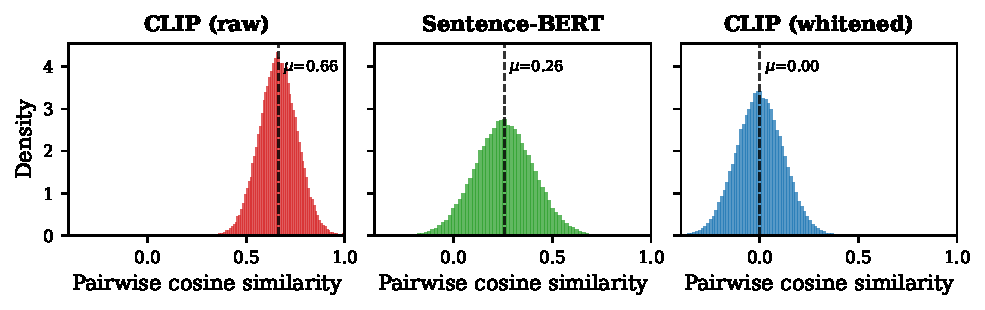
\includegraphics[width=\linewidth]{figures/cosine_histograms.pdf}
\caption{Pairwise cosine similarity distributions of teacher embeddings on AudioCaps captions.
\textbf{Left:} Raw CLIP text embeddings collapse into a narrow cone (mean cosine 0.66).
\textbf{Center:} Sentence-BERT embeddings are well-spread (mean 0.25).
\textbf{Right:} Whitened CLIP embeddings are centered at 0.00, matching SBERT's spread.
The cone collapse explains why raw CLIP fails at distillation: the student cannot distinguish semantically different captions when all teacher embeddings point in nearly the same direction.}
\label{fig:cosine_hist}
\end{figure}

\begin{figure}[t]
\centering
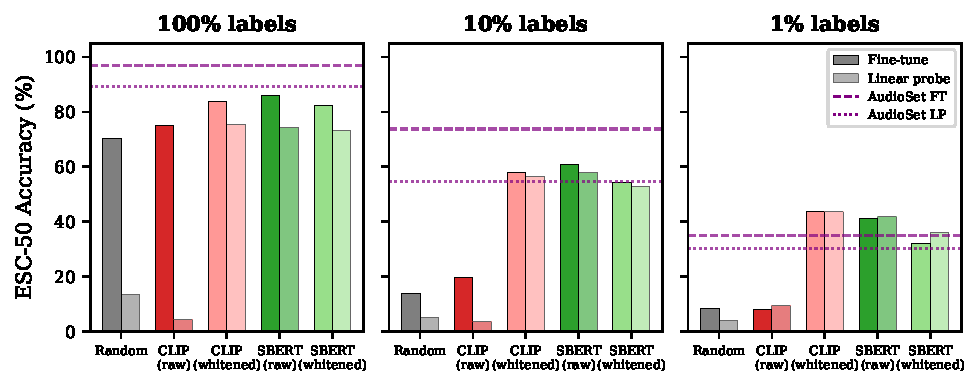
\includegraphics[width=\linewidth]{figures/esc50_bar.pdf}
\caption{ESC-50 accuracy across all conditions. Dashed lines show AudioSet-pretrained performance. At 1\% labels, both CLIP-whitened and SBERT-distilled students exceed the AudioSet ceiling despite training on 46K text-audio pairs vs.\ 2M AudioSet clips. Whitening transforms raw CLIP (near-random) to match SBERT.}
\label{fig:bar}
\end{figure}

%% ============================================================
\section{Discussion}
\label{sec:discussion}

\paragraph{Evidence for the platonic hypothesis.}
Three findings support convergent representations:
(1) After whitening, CLIP and Sentence-BERT---trained with different objectives, architectures, and data---produce identical downstream utility when distilled into tiny audio models.
(2) CLIP's geometric structure is superior to supervised pretraining (15/15 on linear probing), suggesting multimodal training captures more transferable structure.
(3) Foundation model distillation beats domain-specific pretraining in the low-data regime, even across modalities.

\paragraph{Nuances.}
Structure is necessary but not sufficient: content alignment (cosine loss) dominates structural alignment (CKA), with CKA+cosine winning 52/63 comparisons.
Teacher scale does not help (ViT-L $\approx$ ViT-B downstream), indicating student capacity is the bottleneck.
Fine-tuning convergence speed is not improved---distilled students learn faster only on linear probes, not when the full model adapts.

\paragraph{Linear probing as a geometric diagnostic.}
All of our positive results about representation quality come from linear probing.
Fine-tuning masks geometric differences by adapting the backbone.
We recommend linear probing as the primary evaluation when studying representation geometry, consistent with recent arguments by \citet{maniparambil2024vision}.

\paragraph{Practical recipe.}
Before cross-domain distillation, compute mean pairwise cosine similarity over a sample of teacher embeddings.
If it exceeds $\sim$0.5, apply per-dimension whitening (mean/std normalization + L2 renormalization).
This takes seconds to compute and can recover 40+pp of lost performance.

%% ============================================================
\section{Conclusion}
\label{sec:conclusion}

Foundation model geometry transfers across modalities and survives compression into tiny models.
Cone collapse---where out-of-domain embeddings concentrate in a narrow subspace---can obscure this shared structure, but simple whitening recovers it.
After normalization, models trained with fundamentally different objectives converge to the same downstream utility, providing evidence that the semantic content of foundation model representations is shared even when their coordinate systems differ.

\bibliography{references}
\bibliographystyle{plainnat}

\end{document}
